\documentclass[t]{beamer}

% Load general definitions
% Preamble file - general definitions, package loading, etc.

%=================================
% Load packages
\usepackage{amssymb,amsmath}
\usepackage{graphicx}
\usepackage{url}
\usepackage{tikz}
\usetikzlibrary{mindmap,trees,arrows}
\usepackage{fancyvrb}
\usepackage[portuguese]{babel} 
\usepackage[utf8]{inputenc}
\usepackage{subfigure}
\usepackage{times}
\usepackage[T1]{fontenc}
\usepackage{cancel}
\usepackage{color}
\usepackage{listings}
\usepackage[document]{ragged2e}
\usepackage{hyperref}
\usepackage{listings}


%=================================
% Set mode
\mode<presentation>
{
	\usetheme{Madrid}
	\usecolortheme{structure}
	\useoutertheme{infolines}
	\setbeamercovered{invisible}
}

% Get rid of nav bar
\beamertemplatenavigationsymbolsempty

% Insert frame number at bottom of the page.
\usefoottemplate{\hfil\tiny{\color{black!90}\insertframenumber}} 

%=================================
% Define new commands

\newcommand\Real{{\mathbb{R}}}
%\newcommand{\vi}{\vspace{0.6\baselineskip}}
%\newcommand{\goodgap}{\hspace{\subfigtopskip}\hspace{\subfigbottomskip}}


% Equation environments
\newcommand{\beq}{\begin{equation}}
\newcommand{\eq}{\end{equation}}
\newcommand{\beqs}{\begin{equation*}}
\newcommand{\eqs}{\end{equation*}}
\newcommand{\beqn}{\begin{eqnarray}}
\newcommand{\eqn}{\end{eqnarray}}
% Bold variables
\newcommand{\mbf}[1]{\ensuremath{\mathbf{#1}}}
% Itemization
\newcommand{\bitem}{\begin{itemize}}
\newcommand{\eitem}{\end{itemize}}
\newcommand{\spitem}{\vskip 1em\item}
\newcommand{\bitems}{\begin{itemize}\item}
\newcommand{\benums}{\begin{enumerate}\item}
\newcommand{\eenum}{\end{enumerate}}
% color blocks
\newenvironment{colorblock}[2]{%
\setbeamercolor{block title}{#2}
\begin{block}{#1}}{\end{block}}
% Vertical spacing
\newcommand{\vone}{\vskip 1em}
\newcommand{\vhalf}{\vskip .5em}
% Frame environments
\newenvironment{ftst}[3][t]{%
\begin{frame}{environment=ftst,#1}
\frametitle{#2}
\framesubtitle{#3}}{\end{frame}}
\newenvironment{ftstf}[2]{
\begin{frame}[fragile,environment=ftstf]
\frametitle{#1}
\framesubtitle{#2}}{\end{frame}}
% colors
\definecolor{MyGray}{rgb}{0.5,0.5,0.5}
\definecolor{MyDBGray}{rgb}{0.1,0.1,0.4}
\definecolor{darkgreen}{rgb}{0,0.4,0}
\definecolor{black}{rgb}{0,0,0}
\def\defn#1{{\color{red} #1}}
% Footnote
\renewcommand{\thefootnote}{\alph{footnote}}
% Relaxed footnotes
\newcommand{\lfr}[1]{\let\thefootnote\relax\footnote{\tiny #1}}
% Verbatim environment - using FANCYVRB package
\DefineVerbatimEnvironment%
{rcode}{Verbatim}
{fontsize=\scriptsize}

% Verbatim environment - using LISTINGS package
%\lstnewenvironment{rcode} {\lstset{	language = R,
%									basicstyle = \scriptsize\ttfamily,
%									showspaces = false,
%									showstringspaces = false,
%									showtabs = false,
%									keywordstyle = \color{black}\bfseries,
%									commentstyle = \color{darkgreen},
%									numbers = none,
%									otherkeywords={	<-,
%													ggplot,
%													geom_boxplot,
%													facet_grid,
%													shapiro.test,
%													fligner.test,
%													glht,
%													with},
%									deletekeywords={data,
%													model,
%													residuals,
%													c,
%													axis,
%													default,
%													labels,
%													qq.text}}}%
%{}

% Specific definitions
\title[]{Tópicos Especiais em Computação I}
\subtitle[]{Regressão Logística}
\author[]{Patrícia Lucas\\{\footnotesize }}
\institute{Bacharelado em Sistemas de Informação \\ IFNMG  - Campus Salinas}
\date{\scriptsize Salinas\\Abril 2021}

\begin{document}

\setbeamertemplate{caption}{\raggedright\insertcaption\par}
% cover page
\setbeamertemplate{footline}{}
\begin{frame}

\begin{center}
\includegraphics[width=.15\textwidth]{}
\end{center}
  \titlepage
  \begin{tikzpicture}[remember picture,overlay]
  \node[anchor=south east,xshift=-5pt,yshift=5pt] at (current page.south east) {\tiny Versão 1.2021};
  \node[anchor=south west,yshift=0pt] at (current page.south west) {
\includegraphics[width=.25\textwidth]{Logos/salinas_horizontal_jpg.jpg}};
  \end{tikzpicture}  
\end{frame}

% Main slides

\begin{ftst}{Referência}{Regressão Logística}
\begin{figure}
    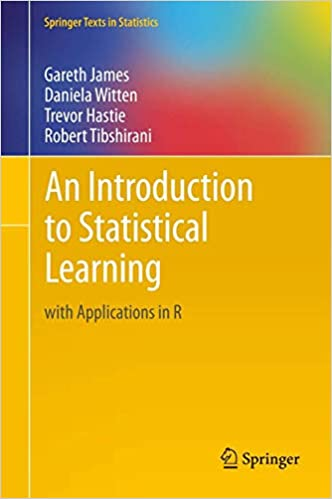
\includegraphics[scale=0.3]{Figuras/slide03_01.jpg}
\end{figure}
Capítulo 4: Logistic Regression
\vone
\scriptsize

An Introduction to Statistical Learning: with Applications in R. G. James, D. Witten, T. Hastie, and R. Tibshirani. Springer, 2013.

\end{ftst}

%=====

\begin{ftst}{Exemplo}{Regressão Logística}
\vone
\begin{figure}
    \centering
    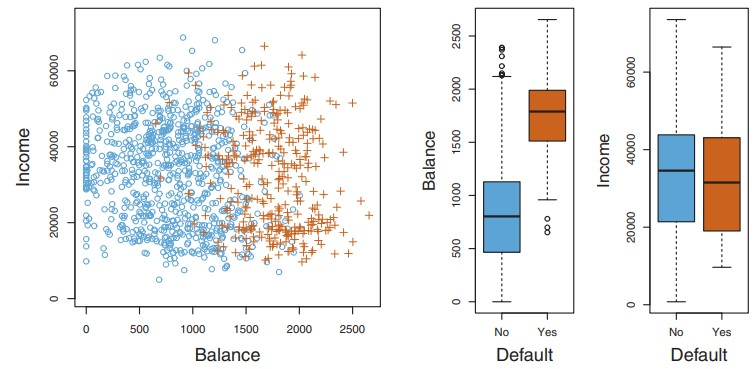
\includegraphics[scale=0.5]{Figuras/slide05_04.jpg}
\end{figure}


\end{ftst}

%=====

\begin{ftst}{Exemplo}{Regressão Logística}
Vamos supor que queremos classificar os clientes como inadimplentes ou não inadimplentes de acordo com o saldo do cartão.
\vone
Ou seja, queremos encontrar uma curva que nos dê a probabilidade de um cliente ser inadimplente com base no seu saldo do cartão.
\begin{equation}
    P(\text{inadimplência}=\text{Sim} | \text{Saldo})
\end{equation}

\begin{figure}
    \centering
    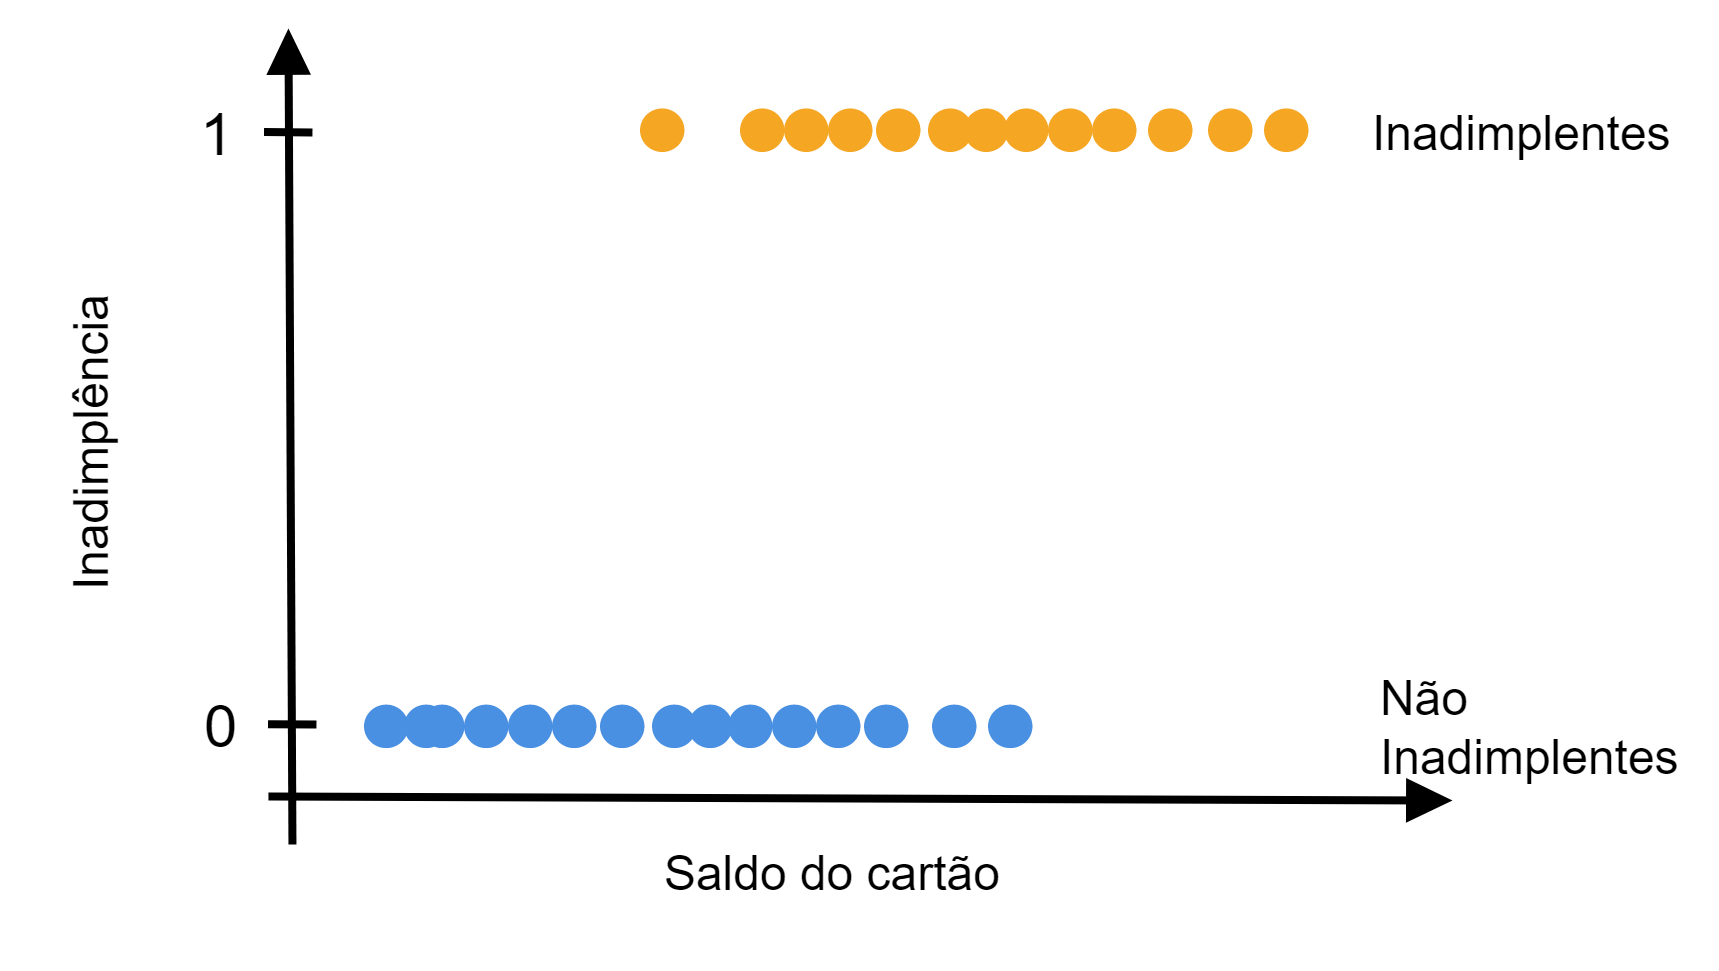
\includegraphics[scale=0.125]{Figuras/slide05_05.png}
\end{figure}


\end{ftst}

%=====

\begin{ftst}{Regressão linear??}{Regressão Logística}
\small
Podemos usar regressão linear para resolver esse problema? 

\begin{enumerate}
    \item Para saldos próximos a zero, prevemos uma probabilidade negativa de inadimplência.
    \item Com saldos muito grandes, obteríamos valores maiores que 1.
\end{enumerate} 

Essas previsões não são sensatas, pois é claro que a verdadeira probabilidade de inadimplência, independentemente do saldo do cartão de crédito, deve cair entre 0 e 1. 

\begin{figure}
    \centering
    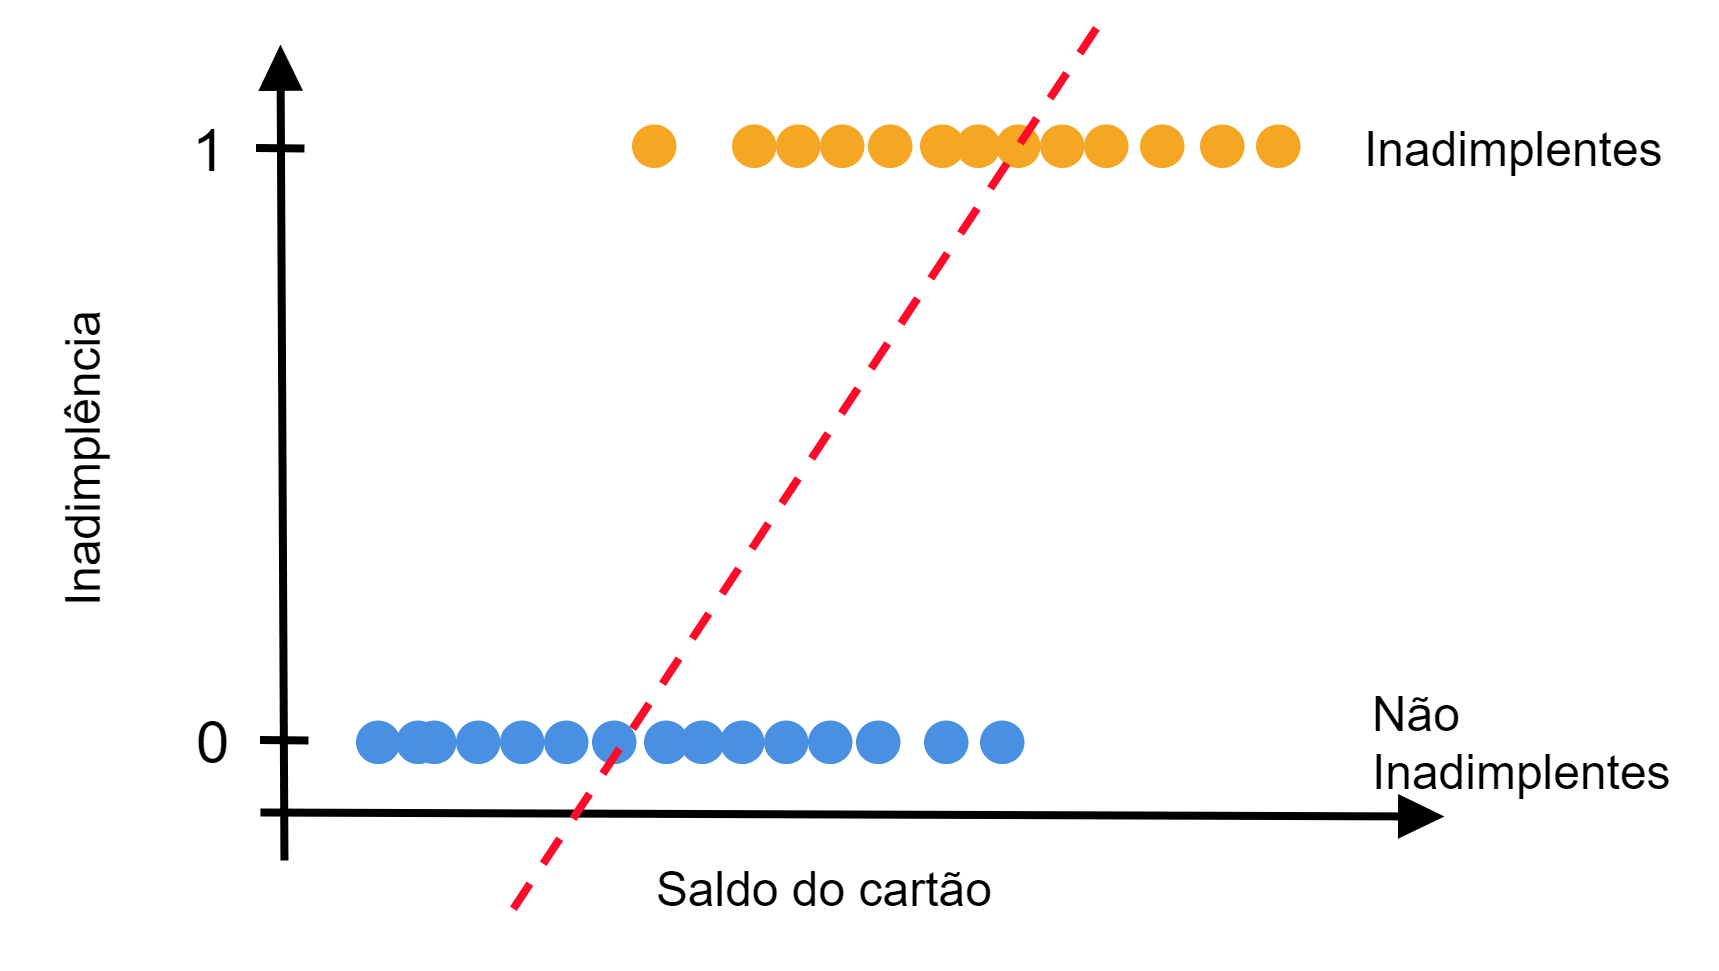
\includegraphics[scale=0.125]{Figuras/slide05_06.png}
\end{figure}

\end{ftst}

%=====

\begin{ftst}{Função logística}{Regressão logística}
\small
Para evitar esse problema, precisamos modelar $P(X)$ usando uma função que fornece saídas entre $0$ e $1$ para todos os valores de $X$. 
\vone
Na regressão logística, usamos a \textbf{função logística}, que ajusta uma curva em “S” que varia entre $0$ e $1$.
\begin{equation}
    P(X) = \frac{\exp{\beta_0 + \beta_1 X}}{1 + \exp{\beta_0 + \beta_1 X}}
\end{equation}

\begin{figure}
    \centering
    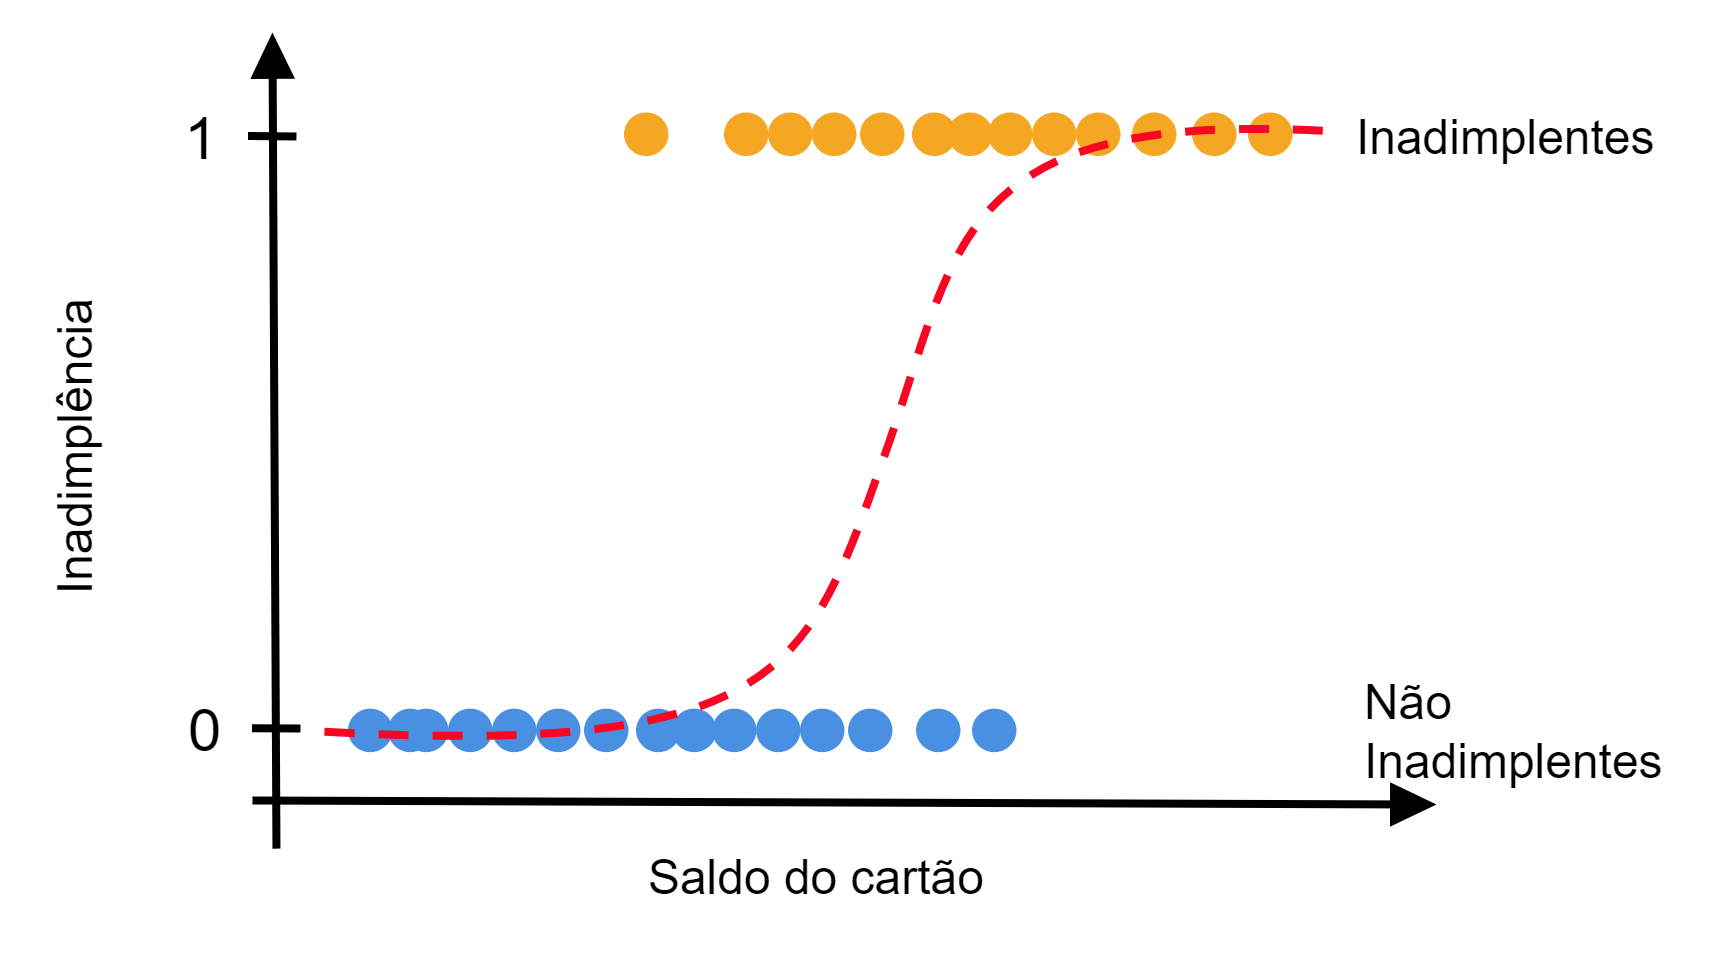
\includegraphics[scale=0.12]{Figuras/slide05_07.png}
\end{figure}


\end{ftst}

%=====

\begin{ftst}{Estimativa dos coeficientes}{Regressão logística}
Os coeficientes $\beta_0$ e $\beta_1$ são desconhecidos e devem ser estimados com base nos dados de treinamento disponíveis. 
\vone
Usamos a abordagem de mínimos quadrados para estimar os coeficientes de regressão linear. Para a regressão logística, usa-se geralmente o método de máxima verossimilhança.
\vone
A intuição básica por trás do método de máxima verossimilhança é tentar encontrar $\beta_0$ e $\beta_1$ de modo que, ao incluir essas estimativas no modelo para $P(X)$, produzam um número próximo de $1$ para todos os indivíduos que são inadimplentes e um número próximo de $0$ para todos os indivíduos que não são.

\end{ftst}

%=====

\begin{ftst}{Estimativa dos coeficientes}{Regressão logística}
\begin{equation}
    l(\beta_0, \beta_1) = \prod_{i:y_i=1} p(x_i) \prod_{i':y_{i'}=0} p(x_{i'})
\end{equation}

\begin{figure}
    \centering
    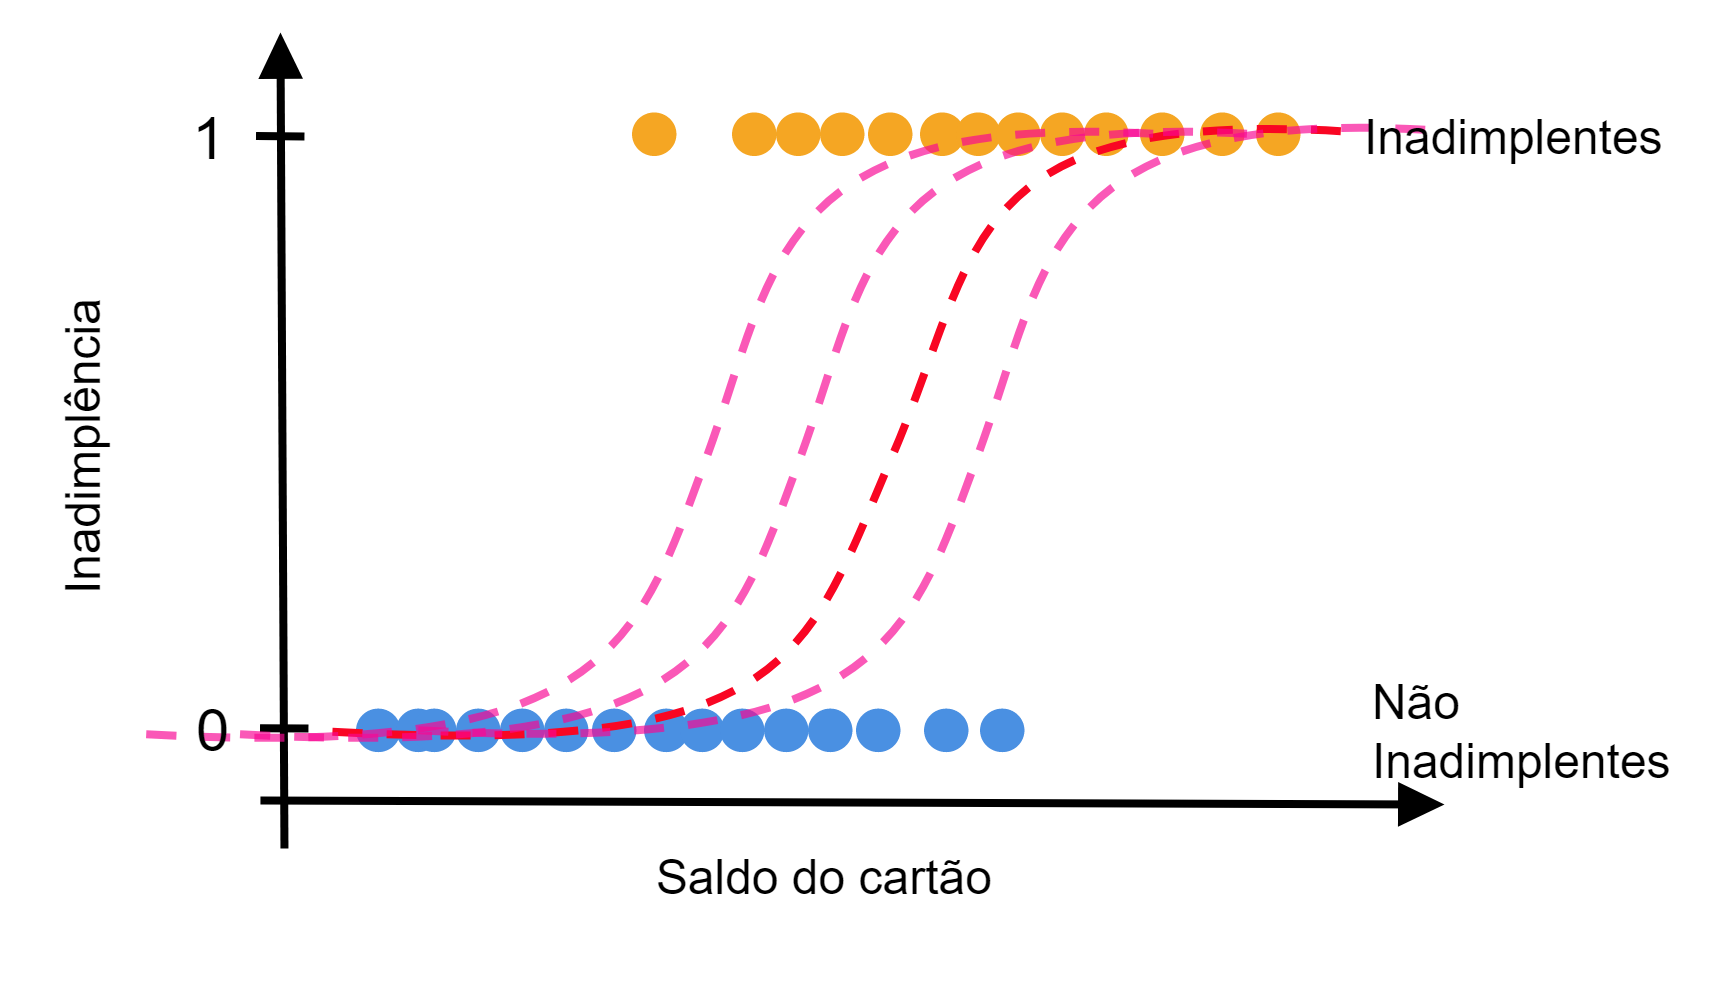
\includegraphics[scale=0.15]{Figuras/slide05_08.png}
\end{figure}


\end{ftst}




\end{document}